% !TEX root = deplump.tex

\begin{figure*}[t] 
	\begin{center}
		\scalebox{.42}{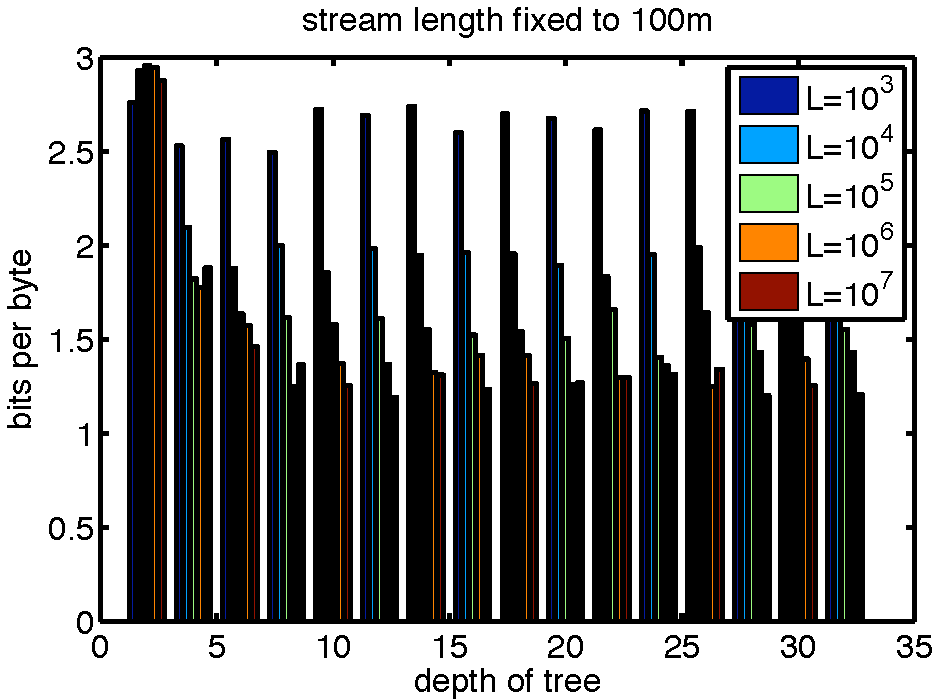
\includegraphics{figs/varying_depths.pdf}} % [clip=true, viewport= 1in 1in 9in 9in]
		\caption{Average ($\pm$ std.) streaming deplump compression performance as measured in bits in compressed output vs.~bytes in uncompressed input.  Here the depth limit ($D$) and node limit ($L$) are varied.  From this we conclude that setting the depth limit to $D\geq16$ and the node limit to the largest value possible given physical memory constraints leads to optimal compression performance.}
		\label{fig:varying_depths}
	\end{center} 
\end{figure*} 

%\begin{figure*}[t] 
%	\begin{center}
%		\scalebox{.6}{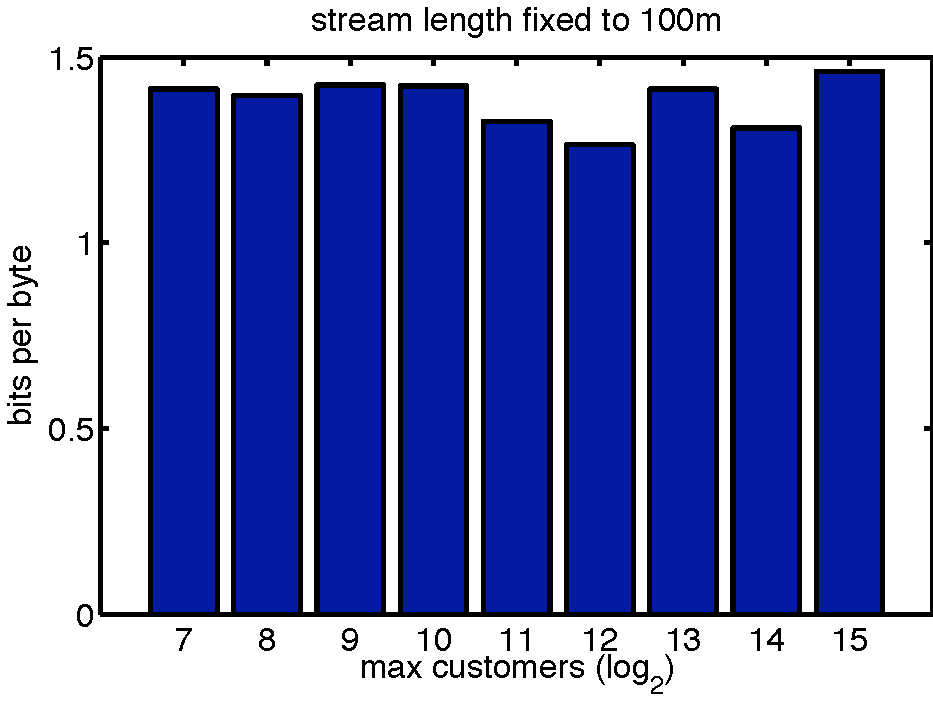
\includegraphics{figs/varying_max_customers.pdf}} % [clip=true, viewport= 1in 1in 9in 9in]
%		\caption{Performance for varying max allowable customers $k$.}
%		\label{fig: varying_max_customers}
%	\end{center} 
%\end{figure*} 

\begin{figure*}[t] 
	\begin{center}
		\scalebox{.42}{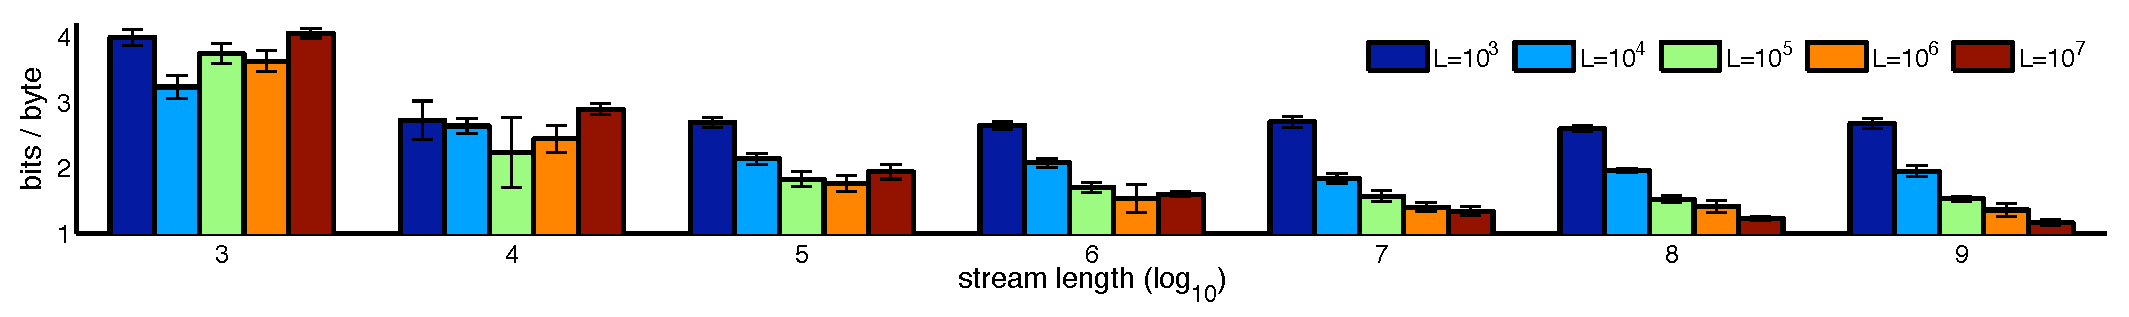
\includegraphics{figs/varying_stream_length.pdf}} % [clip=true, viewport= 1in 1in 9in 9in]
		\caption{Average ($\pm$ std.) streaming deplump compression performance as measured in bits in compressed output vs.~bytes in uncompressed input.  Here the input stream length and node limit ($L$) are varied.  From this we observe that average deplump streaming compression performance monotonically improves as the input sequence grows in length but asymptotes at a different value per node limit  Also, it can be seen that large node limits may actually hurt compression performance for small input sequences.}
		\label{fig:varying_stream_length}
	\end{center} 
\end{figure*} 

\section{Experiments}
\label{sec:experiments}

As the performance of batch deplump was established relative to other lossless compressors for a variety of datatypes in \citep{Gasthaus2010}, we focus our experiments on establishing a) that the approximations to inference in the sequence memoizer combined in this paper in order to make deplump a streaming compressor do not significantly adversely affect compression performance, b) that the resulting compressor can indeed compress extremely long sequences as the asymptotic guarantees would suggest it should, and c) which settings of the approximation parameters produce the best compression performance.

Almost all of the experiments included in this paper use a complete Wikipedia text content dump \citep{Wikipedia2010} as a test corpus (26.8Gb uncompressed, 7.8Gb gziped and ??Gb paq9a'ed, each with default parameters, and 3.9Gb deplumped).  

To establish what approximation parameters produce the best compression results we first ran streaming deplump on the first 100Mb section of the corpus limiting the depth to two different values ($D=16$ and $D=1024$) with a fixed limit on the number of nodes in the tree ($L=10^6$).  We observed that in both cases only very few nodes had high total counts ($c > 8,192$) suggesting that it might be possible to set the count upper bound conservatively ($k= 8,192$) without significant compression performance degradation.  %That compression performance should not be affected by a reasonable count bound follows intuitively from the fact that in byte sequences $|\Sigma| = 256$ and setting $k=10,000$ is similar in effect to using 10,000 observations to estimate a 256 element discrete distribution.  
To ensure that compression performance did in fact not suffer, we compressed ten 100Mb subsections of the corpus (sampled randomly with replacement) for multiple values of $k$ between 128 and 32,768 (fixing $L=10^6$ and $D=16$).  We observed that average compression performance indeed varied insignificantly over all values of $k$.

  In the next experiment, the interplay between limiting the number of nodes in the tree and restricting the depth of the tree was explored (results for which are shown in Figure~\ref{fig:varying_depths}).  Here $k$ was set to 8,192, while $L$ and the depth of the tree $D$ were varied as indicated in the figure.  In another experiment, the interplay between stream length and node limit was explored (Figure~\ref{fig:varying_stream_length}).  In this experiment $k$ remained fixed at the same value and the depth was set to $D=16$ while $L$ varied as shown in the figure.  
 In both experiments, subsections of the corpus were sampled with replacement.  In the first experiment the sampled subsections were all of size 100Mb, while in the second the sampled subsections varied in length.

Figure~\ref{fig:varying_depths} indicates that compression performance becomes essentially indistinguishable for depth restrictions greater than $D=10$.  However, this figure also suggests that compression performance almost improves as a function of the number of nodes in the tree for depths 6 and greater.  Figure~\ref{fig:varying_stream_length} illustrates that the algorithm not only scales to very long sequences, but average compression performance continues to improve as the sequence grows.  Using a large value of $L$ appears to be beneficial for very long sequences.


Considering these results, we chose seemingly reasonable values for the approximating parameters ($D=16$, $L=10^7$, $k=8,192$, $T=10^8$, $\mathcal{D} = [.5, .6, .7, .8, ..., .1]$, and $\eta=??$) then compared streaming deplump to to batch deplump.  In this experiment we compressed the 100Mb Wikipedia corpus excerpt used for the Hutter Prize \citep{Hutter2006} using the streaming variant of deplump and found it gives a compression ratio of 4.78.  Using batch deplump gives a compression ratio of 4.82 \citep{Gasthaus2010}, while running batch deplump repeatedly on the 5Mb subsections of the corpus reduces the compression ratio to 4.25.  These results demonstrate that the approximations made for streaming deplump give it a significant advantage over compressing the file in chunks and have very little negative effect when compared to the full model.




%\begin{figure*}[t] 
%	\begin{center}
%		\scalebox{1}{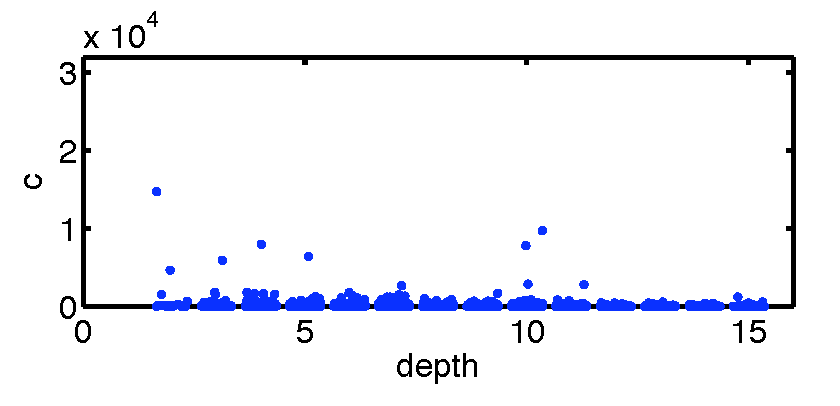
\includegraphics{figs/scatter_16.pdf}} % [clip=true, viewport= 1in 1in 9in 9in]
%		\caption{Scatter plots to explore the relationship between the depth of a node and the total count}
%		\label{fig:restaurant_plots}
%	\end{center} 
%\end{figure*} 

%\begin{figure*}[t] 
%	\begin{center}
%		\scalebox{1}{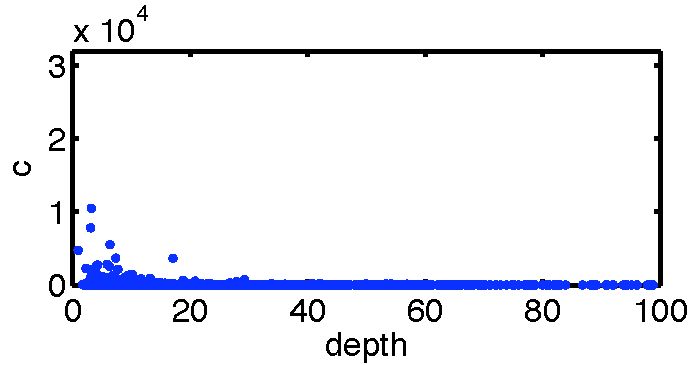
\includegraphics{figs/scatter_1024.pdf}} % [clip=true, viewport= 1in 1in 9in 9in]
%		\caption{Scatter plots to explore the relationship between the depth of a node and the total count}
%		\label{fig:restaurant_plots}
%	\end{center} 
%\end{figure*} 
